\documentclass{article}
\usepackage[margin=2.6cm]{geometry}
\usepackage{graphicx}
\usepackage{booktabs}
\usepackage{amsmath}
\usepackage{hyperref}
\usepackage{float}
\usepackage{caption}
\usepackage{subcaption}
\usepackage{xcolor}

\title{Case 2: Low-Dimensional Representation and Latent State Discovery in Wearable Biosignals}
\author{02582 Computational Data Analysis\\s252646}
\date{}

\begin{document}
\maketitle

\begin{abstract}
This report investigates whether physiological features from the EmoPairCompete dataset reveal subject-invariant emotional or stress-related states. We use the provided heart rate, skin temperature, and electrodermal activity features as the primary data source and evaluate three preprocessing choices: global standardization, subject-wise normalization, and subtraction of the pre-puzzle resting baseline. Principal component analysis (PCA) is used to derive low-dimensional representations, and KMeans clustering is used to test whether latent clusters align with the three experimental phases. The main finding is a negative but informative result: the raw representation is dominated by individual and cohort effects, while phase explains only a small part of the variance. Subject-wise normalization increases the phase-related structure, but unsupervised clustering still does not reliably recover the experimental phases. A supervised leave-one-subject-out sanity check suggests that some phase1/phase2 signal exists, but the signal is too weak and baseline-dependent for simple unsupervised discovery. This supports the interpretation that wearable biosignal representations require careful normalization and rigorous validation before being treated as emotional state detectors.
\end{abstract}

\section*{Introduction and Research Questions}
Wearable physiological sensors provide continuous measurements that may reflect stress, frustration, or recovery. However, signals such as heart rate (HR), electrodermal activity (EDA), and skin temperature (TEMP) are also strongly affected by individual baselines, device placement, time of day, and measurement noise. This makes the EmoPairCompete dataset a realistic setting for testing whether computational data analysis methods can derive meaningful emotional representations from noisy biosignals.

We focus on the ``Representation Challenge'' and combine it with latent state discovery. Our aim is not only to visualize the data, but to test whether a low-dimensional representation contains phase-related structure after accounting for subject-specific baselines. The analysis is guided by three research questions:

\begin{enumerate}
    \item Are the dominant directions of variation in the biosignal features related to the experimental phase, or are they mainly driven by individual and cohort effects?
    \item Does subject-wise normalization or baseline subtraction improve the phase-related structure in a PCA representation?
    \item Do unsupervised clusters in the low-dimensional space correspond to the known experimental phases: pre-puzzle rest, puzzle task, and post-puzzle rest?
\end{enumerate}

The expected outcome is not necessarily a clean separation of emotional states. The dataset description explicitly notes that wearable biosignals are noisy and baseline-dependent. Therefore, a rigorous null result is meaningful if the pipeline makes clear what was tested and why the evidence does or does not support latent emotional state discovery.

\section*{Data Description}
The dataset consists of physiological recordings from the Empatica E4 wristband collected during a competitive tangram puzzle experiment. Each participant completed four rounds. Every round contains three phases: phase1, a pre-puzzle resting period; phase2, the puzzle competition; and phase3, a post-puzzle resting period. After each phase, participants answered self-report questions including frustration and PANAS-style affect items.

We used the updated feature file \texttt{HR\_data\_2.csv}. It contains 312 observations, corresponding to 26 individuals, four rounds, and three phases per round. The input feature set contains 51 pre-extracted physiological features from HR, TEMP, and EDA. Metadata and questionnaire variables such as \texttt{Phase}, \texttt{Individual}, \texttt{Cohort}, \texttt{Puzzler}, and \texttt{Frustrated} were not used as input features. They were used only for interpretation and validation.

The feature matrix contained only two missing values, both in EDA rise/recovery-time features. These were imputed using the median. Across the full file there were nine missing values, but the additional missing entries were in self-report variables and did not affect PCA or clustering. The target labels were balanced across phases: 104 observations in each phase.

\section*{Methods}
\subsection*{Preprocessing}
Let $X \in \mathbb{R}^{n \times p}$ denote the physiological feature matrix, with $n=312$ observations and $p=51$ features. We compared three preprocessing pipelines.

\paragraph{Raw scaled features.}
Missing feature values were median-imputed, and each feature was standardized to zero mean and unit variance:
\[
z_{ij} = \frac{x_{ij} - \mu_j}{\sigma_j}.
\]
This is the simplest representation, but it does not correct for individual physiological baselines.

\paragraph{Subject-wise normalization.}
For each individual $s$, each feature was centered and scaled using only that individual's observations:
\[
z_{isj} = \frac{x_{isj} - \bar{x}_{sj}}{s_{sj}}.
\]
This removes static between-subject differences and tests whether within-subject changes contain phase-related information.

\paragraph{Phase1 baseline subtraction.}
For each individual and round, we subtracted the corresponding phase1 value:
\[
\Delta x_{srpj} = x_{srpj} - x_{sr,\mathrm{phase1},j}.
\]
This represents phase2 and phase3 as deviations from the pre-puzzle resting baseline within the same round. It is motivated by the fact that biosignals often need a personal baseline to be interpretable.

\subsection*{PCA Representation}
PCA was used to derive low-dimensional representations from each preprocessed feature matrix. PCA finds orthogonal directions $w_k$ that maximize projected variance:
\[
\max_{\|w_k\|=1} \mathrm{Var}(Xw_k).
\]
We used the first five principal components (PCs) for downstream evaluation because they captured a substantial fraction of the variance while avoiding excessive high-dimensional noise.

To quantify what drives the PCA representation, we computed a weighted $R^2$ between the first five PC scores and four metadata variables: phase, individual, cohort, and puzzler role. For each metadata variable, a least-squares model predicted the PC scores from one-hot encoded labels. The per-PC $R^2$ values were then averaged using each PC's explained variance as weight. This is not a predictive model; it is a diagnostic measure of how much low-dimensional variance is associated with each known factor.

\subsection*{Latent State Discovery}
We applied KMeans clustering to the first five PC scores using $k=3$, matching the number of experimental phases. KMeans minimizes the within-cluster sum of squared distances:
\[
\min_{\{C_k\}, \{\mu_k\}} \sum_{k=1}^{K} \sum_{i \in C_k} \|z_i - \mu_k\|_2^2.
\]
The clusters were evaluated against the known phase labels using adjusted Rand index (ARI), normalized mutual information (NMI), and a cluster-by-phase heatmap. Silhouette score was also reported as an internal clustering measure. A high silhouette score alone is not sufficient, because clusters may reflect individual baselines or cohorts rather than emotional states.

\subsection*{Sanity Checks}
As a secondary check, we evaluated two alternatives. First, a one-class SVM was trained only on phase1 observations in a leave-one-subject-out (LOSO) setting and then tested on held-out subjects. This tests whether puzzle and recovery phases appear anomalous relative to resting data. Second, a supervised logistic regression classifier was trained to distinguish phase2 from phase1 under LOSO validation. This supervised analysis was not used as the main solution; it only tests whether any generalizable phase signal exists at all.

\section*{Results}
\subsection*{Raw Features Are Dominated by Subject and Cohort Effects}
The raw scaled PCA representation showed that the first five PCs explained 58.4\% of the total feature variance. However, the dominant structure was not phase-related. Individual identity explained 64.5\% of the weighted variance in PC1-PC5, and cohort explained 32.8\%. In contrast, experimental phase explained only 3.0\%, and puzzler role explained 0.5\%.

\begin{figure}[H]
    \centering
    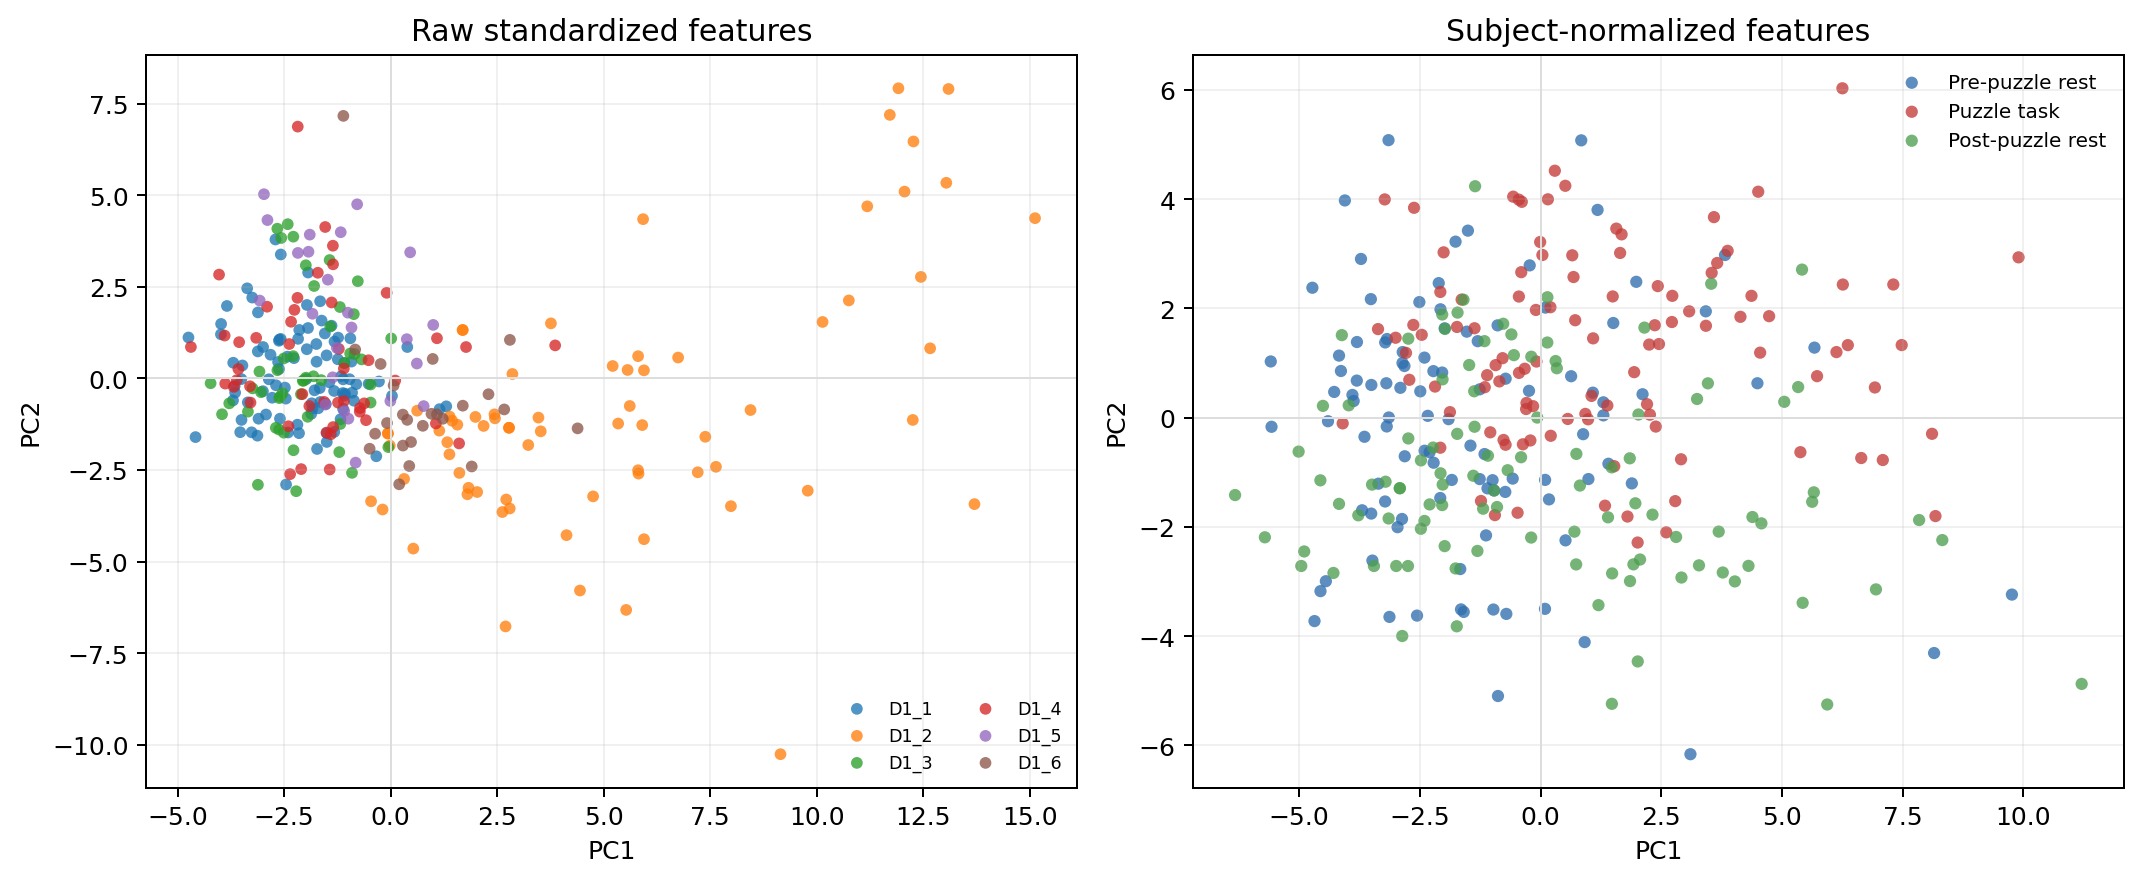
\includegraphics[width=\textwidth]{figures/figure1_pca_comparison.png}
    \caption{Left: PCA on raw standardized features, colored by cohort. Right: PCA on subject-normalized features, colored by phase. Raw features show clear cohort structure, while subject normalization removes much of this baseline effect but still does not produce clean phase separation.}
    \label{fig:pca}
\end{figure}

Figure \ref{fig:pca} illustrates this pattern. In the raw representation, one cohort forms a visibly shifted structure, indicating that acquisition context and individual baselines have a large influence on the features. After subject-wise normalization, the cohort structure is reduced, and phase2 observations become somewhat more dispersed, but the three experimental phases still overlap substantially.

\subsection*{Subject Normalization Improves Phase Signal but Does Not Solve Separation}
Subject-wise normalization increased the weighted phase-related $R^2$ from 3.0\% to 9.9\%. This confirms that removing individual baselines is important. However, even after this correction, most of the variation in the first PCs remains unrelated to phase labels.

\begin{figure}[H]
    \centering
    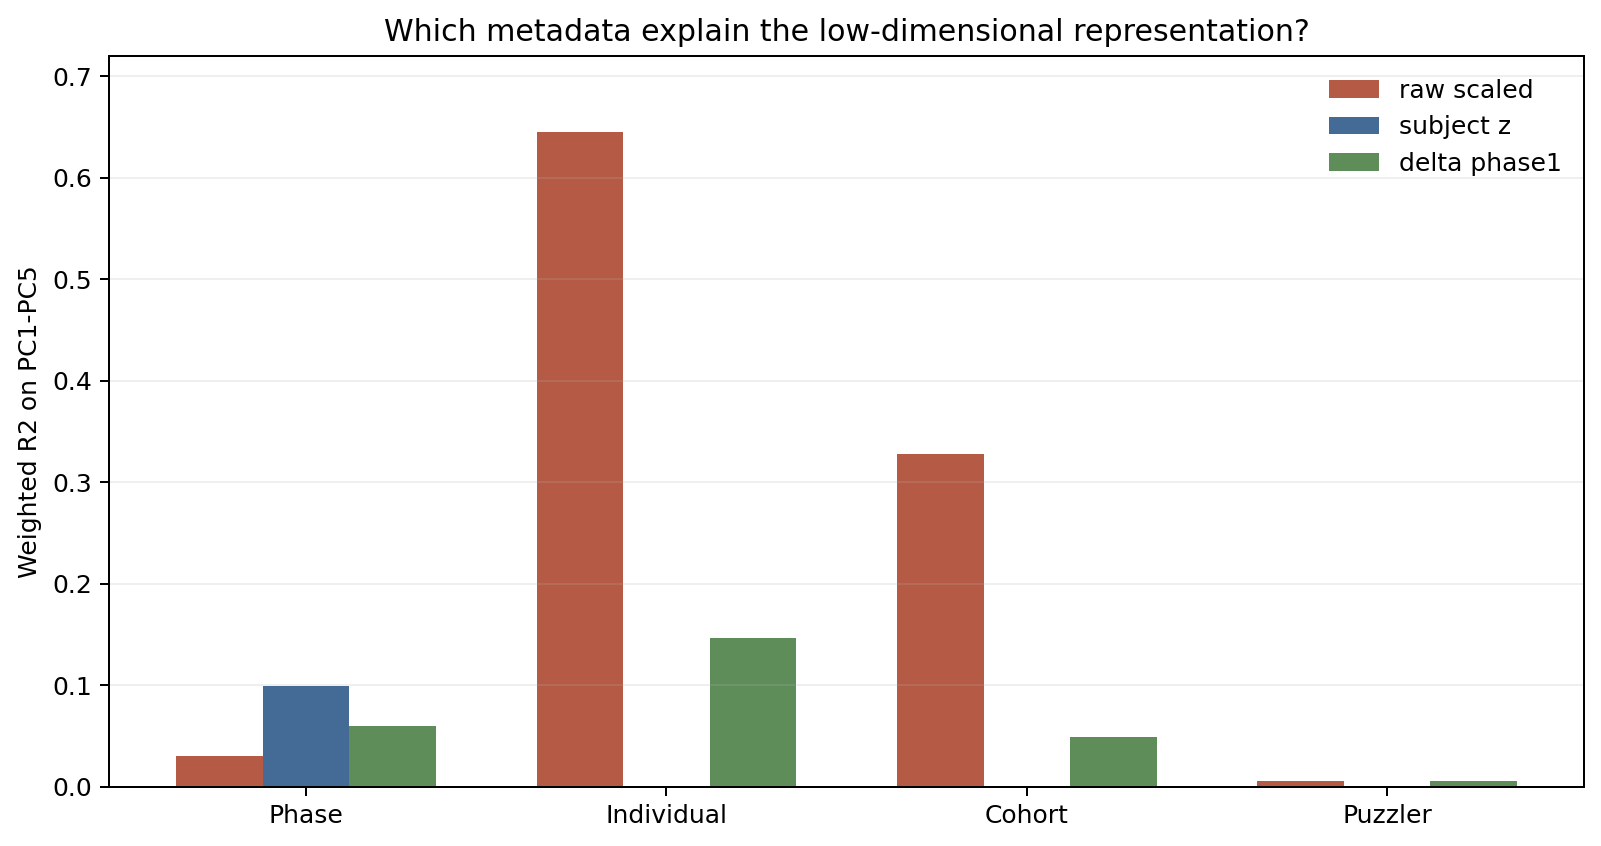
\includegraphics[width=0.86\textwidth]{figures/figure2_metadata_r2.png}
    \caption{Weighted $R^2$ of metadata variables for PC1-PC5. Raw features are dominated by individual and cohort effects. Subject normalization removes static individual/cohort effects and increases the relative contribution of phase, but the phase signal remains weak.}
    \label{fig:r2}
\end{figure}

Baseline subtraction also reduced cohort effects but did not produce as strong a phase signal as subject-wise normalization. Its weighted phase-related $R^2$ was 6.0\%, while individual identity still explained 14.6\%. This suggests that round-level baseline subtraction is useful but may be unstable because phase1 itself is noisy and may contain carry-over effects from previous rounds.

\begin{table}[H]
\centering
\caption{PCA and KMeans summary for the three preprocessing pipelines.}
\begin{tabular}{lrrrrrr}
\toprule
Pipeline & PC1 & PC2 & PC1-PC5 & Silhouette & ARI & NMI \\
\midrule
Raw scaled & 0.278 & 0.100 & 0.584 & 0.320 & -0.003 & 0.004 \\
Subject-wise z & 0.203 & 0.091 & 0.514 & 0.162 & 0.075 & 0.079 \\
Phase1 delta & 0.163 & 0.097 & 0.493 & 0.442 & 0.051 & 0.129 \\
\bottomrule
\end{tabular}
\label{tab:model}
\end{table}

\subsection*{Unsupervised Clusters Do Not Recover Experimental Phases}
KMeans clustering on the first five PCs did not recover the three phases reliably. For raw scaled features, the ARI was approximately zero ($-0.003$), indicating no meaningful agreement with phase labels. Subject-wise normalization improved ARI to 0.075, and phase1 baseline subtraction gave ARI 0.051. These values are still low and indicate weak alignment.

\begin{figure}[H]
    \centering
    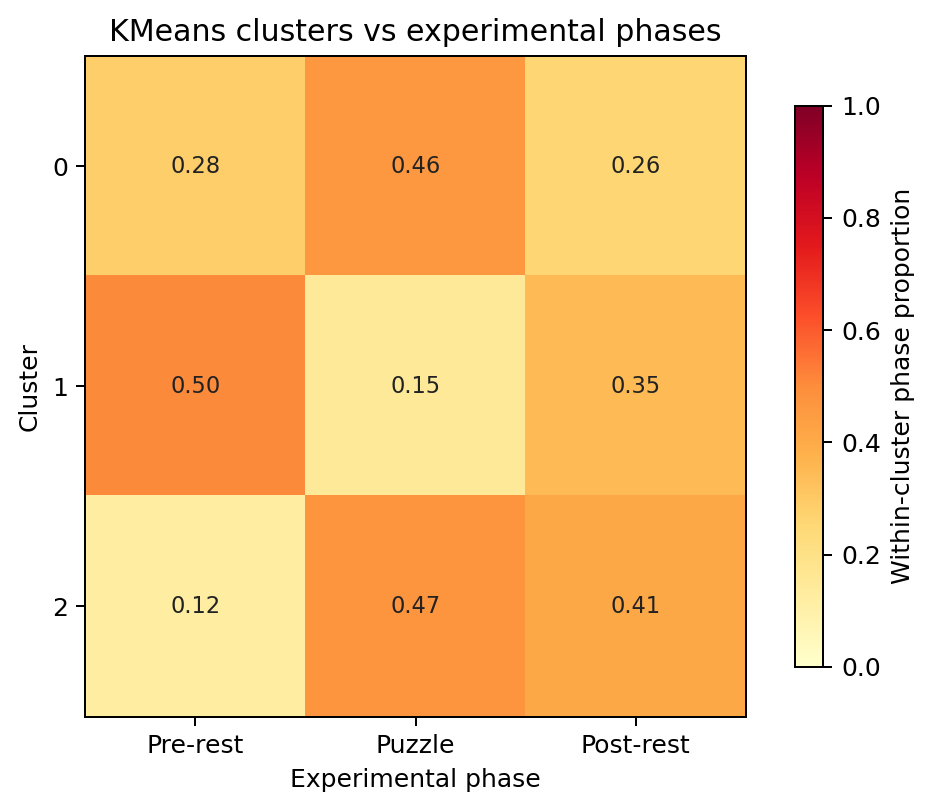
\includegraphics[width=0.58\textwidth]{figures/figure3_cluster_phase_heatmap.png}
    \caption{KMeans clusters from the subject-normalized PCA representation. The clusters contain mixtures of phases rather than one cluster per experimental phase.}
    \label{fig:cluster}
\end{figure}

The heatmap in Figure \ref{fig:cluster} shows that clusters are not phase-pure. One cluster contains more puzzle-task observations, but the separation is not strong enough to interpret the clusters as latent emotional states. This is an important distinction: the data can form geometric clusters, but those clusters do not necessarily correspond to the experimental manipulation.

\subsection*{Sanity Checks}
The one-class SVM trained on phase1 resting data did not successfully flag phase2 as anomalous under LOSO validation. With $\nu=0.10$, phase2-vs-phase1 AUC was 0.402 and balanced accuracy was 0.404. The anomaly rate was actually lower for phase2 than for phase1, which indicates that this simple zero-shot formulation is not reliable for this feature set.

In contrast, a supervised logistic regression sanity check for phase2 versus phase1 achieved LOSO AUC of 0.779, balanced accuracy of 0.692, and F1 score of 0.701. This means the data are not completely uninformative. Some generalizable stress-related signal exists, but it is not strong or structured enough for simple PCA plus KMeans, or for one-class SVM trained only on resting data, to recover clean latent states.

\begin{figure}[H]
    \centering
    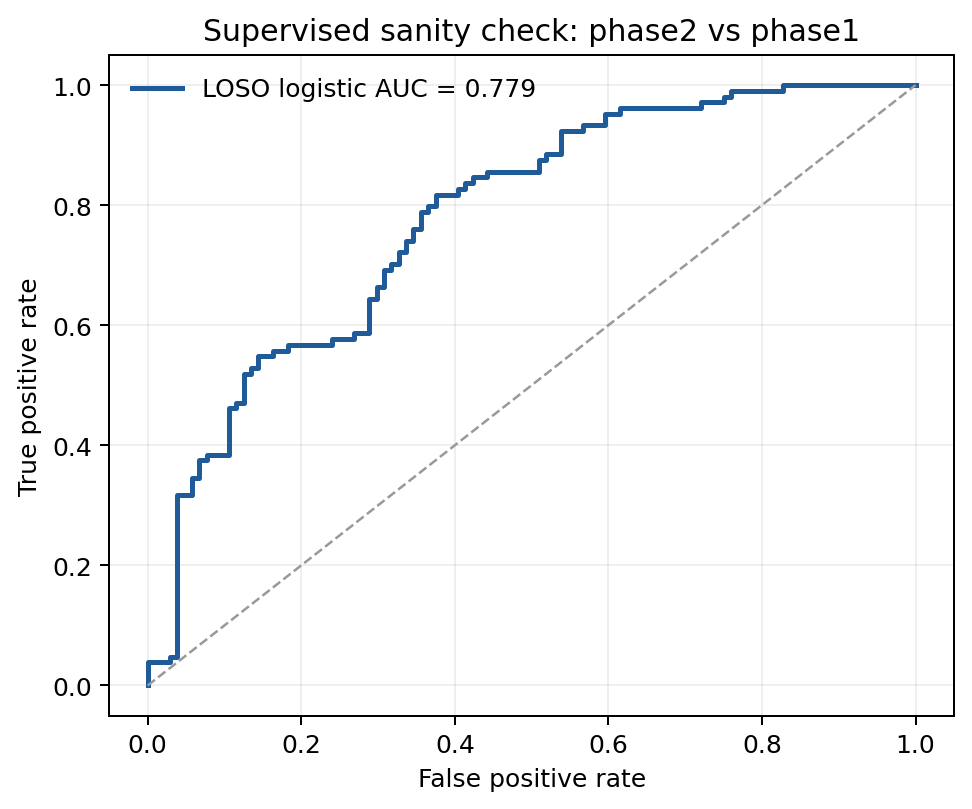
\includegraphics[width=0.58\textwidth]{figures/figure4_supervised_sanity_roc.png}
    \caption{Supervised sanity check for phase2 versus phase1 using LOSO logistic regression. The AUC suggests that some phase-related signal exists, even though unsupervised clustering does not recover the phases cleanly.}
    \label{fig:roc}
\end{figure}

\section*{Discussion}
The main conclusion is that individual baselines are the dominant source of variation in the raw wearable biosignal features. This is expected for HR, TEMP, and EDA because absolute levels differ substantially across people and recording sessions. Without normalization, a latent representation mostly captures who was measured and when the data were collected, not what experimental state the person was in.

Subject-wise normalization is therefore not an optional preprocessing detail; it changes the scientific interpretation of the representation. It removes static individual and cohort effects and increases the amount of phase-related structure. However, the improvement is limited. The phases still overlap in PCA space, and KMeans clusters remain mixtures of pre-rest, puzzle, and post-rest observations. This supports a cautious interpretation: the dataset contains weak stress-related signal, but it does not support strong unsupervised claims about three clearly separable emotional states using this pipeline.

The supervised sanity check is useful because it prevents over-interpreting the negative clustering result. If even a supervised LOSO classifier failed, we might conclude that the feature set contains almost no phase information. Instead, logistic regression achieved AUC 0.779, suggesting that phase information exists but is subtle and distributed across features. Unsupervised methods may fail because the stress signal is not the largest source of variance, whereas PCA explicitly prioritizes high-variance directions. This is a methodological limitation of PCA for stress discovery: the most physiologically dominant variation is not necessarily the most task-relevant variation.

\section*{Limitations}
Several limitations should be considered. First, the sample size is small: 26 individuals and only 12 observations per individual. Second, the feature matrix uses summary statistics over phases, which may discard temporal dynamics within the five-minute windows. Third, cohort effects are strong, and the cohorts were collected at different times and contexts. Fourth, self-reported frustration is subjective and does not necessarily align one-to-one with physiological arousal. Finally, KMeans assumes roughly spherical clusters and may be poorly matched to biosignal manifolds. Future work could use time-series features, mixed-effects models, domain-adversarial normalization, or self-supervised embeddings evaluated under LOSO validation.

\section*{Conclusion}
This case study shows that the EmoPairCompete biosignals contain weak but nonzero phase-related information, but the dominant structure in the raw data is individual and cohort variability. Subject-wise normalization improves the representation, yet unsupervised PCA plus KMeans does not reliably discover latent states corresponding to pre-puzzle rest, puzzle stress, and post-puzzle recovery. The most defensible conclusion is therefore methodological: wearable biosignal analysis requires baseline-aware preprocessing and validation against subject-level generalization before latent emotional clusters can be interpreted as meaningful stress states.

\section*{Reproducibility}
The analysis was implemented in Python using median imputation, standardization, PCA, KMeans, one-class SVM, logistic regression, and leave-one-subject-out validation. The script \texttt{submission/case2\_analysis.py} reads \texttt{HR\_data\_2.zip}, generates all figures, and exports the numerical result tables used in this report.

\section*{GenAI Acknowledgement}
Answer by replacing \textit{[your answer here]} with your response.
\begin{enumerate}
    \item \textit{I abide by \href{https://student.dtu.dk/en/exam/exam-cheating/dtu-code-of-honour}{DTU's code of honour} and take full responsibility for the content of this submission (yes / no)}:
    \begin{itemize}
        \item {[yes]}
    \end{itemize}
    \item \textit{To what extent did you use generative AI to solve this assignment (0-100\%)}:
    \begin{itemize}
        \item {[20]}
    \end{itemize}
    \item \textit{What was the primary use of generative AI, if any (writing / coding / other)}:
    \begin{itemize}
        \item {[writing]}
    \end{itemize}
    \item \textit{I feel I understand the key techniques/algorithms/methods/coding elements used in this exercise such that I can apply it in a \textbf{no aids} exam (yes/no)}:
    \begin{itemize}
        \item {[yes]}
    \end{itemize}
\end{enumerate}

\begin{thebibliography}{9}
\bibitem{das2024}
Das, S., Lund, N. L., Gonzalez, C. R., Lonfeldt, N. N., and Clemmensen, L. H. EmoPairCompete - physiological signals dataset for emotion and frustration assessment under team and competitive behaviors. ICLR Workshop on Learning from Time Series for Health, 2024.

\bibitem{thompson2007}
Thompson, E. R. Development and validation of an internationally reliable short-form of the Positive and Negative Affect Schedule (PANAS). Journal of Cross-Cultural Psychology, 38(2), 227-242, 2007.
\end{thebibliography}

\end{document}
